%; whizzy chapter
% -initex iniptex -latex platex -format platex -bibtex jbibtex -fmt fmt
% 以上 whizzytex を使用する場合の設定。

%     Tokyo Debian Meeting resources
%     Copyright (C) 2011 Junichi Uekawa
%     Copyright (C) 2011 Nobuhiro Iwamatsu

%     This program is free software; you can redistribute it and/or modify
%     it under the terms of the GNU General Public License as published by
%     the Free Software Foundation; either version 2 of the License, or
%     (at your option) any later version.

%     This program is distributed in the hope that it will be useful,
%     but WITHOUT ANY WARRANTY; without even the implied warranty of
%     MERCHANTABILITY or FITNESS FOR A PARTICULAR PURPOSE.  See the
%     GNU General Public License for more details.

%     You should have received a copy of the GNU General Public License
%     along with this program; if not, write to the Free Software
%     Foundation, Inc., 51 Franklin St, Fifth Floor, Boston, MA  02110-1301 USA

%  preview (shell-command (concat "evince " (replace-regexp-in-string "tex$" "pdf"(buffer-file-name)) "&"))
% 画像ファイルを処理するためにはebbを利用してboundingboxを作成。
%(shell-command "cd image201201; ebb *.png")

%%ここからヘッダ開始。

\documentclass[mingoth,a4paper]{jsarticle}
\usepackage{monthlyreport}

% 日付を定義する、毎月変わります。
\newcommand{\debmtgyear}{2012}
\newcommand{\debmtgmonth}{2}
\newcommand{\debmtgdate}{18}
% (+ (* (- 2012 2005) 12) 1 -1) started from zero
\newcommand{\debmtgnumber}{85}

\begin{document}

\begin{titlepage}
\thispagestyle{empty}
% タイトルページ:編集必要な部分は最初のマクロに飛ばすこと

\vspace*{-2cm}
第\debmtgnumber{}回 東京エリア Debian 勉強会資料\\
\hspace*{-2cm}
\includegraphics[width=210mm]{image201003/debsen.eps}\\
\hfill{}\debmtgyear{}年\debmtgmonth{}月\debmtgdate{}日

% ここはアップデートすること
% 全角文字にしないとフォントのサイズが合わないので注意
\rotatebox{10}{\fontsize{23}{23} {\gt 特集1:Debian開発者のKDE環境あれこれ}}

\rotatebox{10}{\fontsize{23}{23} {\gt 特集2:月刊Debhelper}}

\rotatebox{10}{\fontsize{23}{23} {\gt 特集3:cmakeつかってみる}}
\vspace*{-2cm}
\hfill{}
\includegraphics[height=6cm]{image200502/openlogo-nd.eps}
\end{titlepage}

\dancersection{Introduction}{野島 貴英}

\begin{multicols}{2}
 

 今月のDebian勉強会へようこそ。これからDebianの世界にあしを踏み入れると
 いう方も、すでにどっぷりとつかっているという方も、月に一回Debianについ
 て語りませんか?

 Debian勉強会の目的は下記です。

 \begin{itemize}
 \item \underline{Debian Developer} (開発者)の育成。
 \item 日本語での「\underline{開発に関する情報}」を整理してまとめ、アップデートする。
 \item \underline{場}の提供。
 \begin{itemize}
  \item 普段ばらばらな場所にいる人々が face-to-face で出会える場を提供
	する。
  \item Debian のためになることを語る場を提供する。
  \item Debianについて語る場を提供する。
 \end{itemize}
 \end{itemize}		

 Debianの勉強会ということで究極的には参加者全員がDebian Packageをがりがり
 と作るアクティブな開発者になった姿を妄想しています。情報の共有・活用を通し
 て Debianの今後の能動的な展開への土台として、「場」としての空間を提供す
 るのが目的です。

\end{multicols}

\newpage

\begin{minipage}[b]{0.2\hsize}
 \definecolor{titleback}{gray}{0.9}
 \colorbox{titleback}{\rotatebox{90}{\fontsize{80}{80} {\gt デビアン勉強会} }}
\end{minipage}
\begin{minipage}[b]{0.8\hsize}
\hrule
\vspace{2mm}
\hrule
\begin{multicols}{2}
\tableofcontents
\end{multicols}
\vspace{2mm}
\hrule
\end{minipage}

\dancersection{事前課題}{野島 貴英}

今回の事前課題は以下です:
\begin{enumerate}
 \item 皆さんのDebian desktop環境と、利用にあたって何か工夫があれば200文字以内でアピールください。(contrib目標/未来指向なアピールはさらに絶賛歓迎)
\end{enumerate}
この課題に対して提出いただいた内容は以下です。
\begin{multicols}{2}
{\small
\begin{prework}{ 鈴木崇文 }

gnomeでdesktopを利用しています。
工夫というほどではないですが、便利なツールとしてKDE系のアプリやEBViewを使っています。
リモートデスクトップ(RDP) & VNC 用には、KRDC を使い、スクリーンショット用には KSnapshot を使っています。
あとは英辞郎を購入して、EBViewでいつでも翻訳できるようにしています。
\end{prework}

\begin{prework}{ dictoss(杉本 典充) }

低性能マシンはstartx+icewm、中高性能マシンはgdm+xfce4かgnomeと使い分けています。KDEは最近使ってないです。(KDEは重そうなイメージがある)
カスタマイズしているのは、ページャの個数を6つに増やしている、複数のターミナルを重ならないように同時起動するシェルスクリプトを作り一発で画面をターミナルで埋め尽くせるようにしています。(昔タイル型ウィンドウマネージャ使えばいいのに、とか突っ込まれました)
\end{prework}

\begin{prework}{ yamamoto }

メインに使っているのは、録画サーバも兼ねた Debian squeeze (amd64) です。
外出時は気分次第で、sid の i386 ネットブックと sid の amd64 ノート PC を選んでいます。
どれも、特に何の変てつもない、ただの KDE 環境です。

デスクトップとしての見た目は、壁紙すらデフォルトのままで、改造してませんが、機体としては家の LAN にぶら下がったマシン間を「何か(?)」が行き来する、魔改造スクリプトがいくつか仕込んであり、ものぐさな私にはとっても快適です。
\end{prework}

\begin{prework}{ 野島 貴英 }

GNOME 3.2.2をDebianで利用しています。unstableではもの足りず、experimentalからupgradeして引っ張ってきてます。特にクールなカスタマイズは何もしてないですが、gnome-shellがjavascriptなど解釈できるということから、将来ちょっとしたガジェットぐらい作ってみたいなーと思うこの頃です。あと、gxconsole( \url{http://gnomefiles.org/content/show.php/gxconsole?content=132145} )がGNOME3.2.2になっても、やっぱり欲しかったので、GNOME 3.2.2用に移植したい...
\end{prework}

\begin{prework}{ 日比野 啓 }

普段はタイル型ウィンドウマネージャの XMonad を使っています。
マルチディスプレイに対するサポートが使いやすくてプレゼンのときにも便利で気にいっています。
最近、趣味のプログラミングのメインで使っている言語が Haskell なので、
Haskellでカスタマイズできることも魅力です。
gnome-session との組合せも使ってみましたが、なぜか sid ではうまく動かなくて残念。
あと、画面の上下が狭くなるのが嫌なので、なんとかする方法が知りたい。

\end{prework}

}
\end{multicols}

\dancersection{最近のDebian関連のミーティング報告}{野島 貴英}
\subsection{東京エリアDebian勉強会84回目報告}

% (query-replace-regexp "<.*?>" "")
% (query-replace-regexp "^[	 ]\+" "")

  1月の東京エリアDebian勉強会は久しぶりにあんさんぶる荻窪にて行われました。
上川さんから、Debian勉強会予約システムに関する脆弱性と考察、また、Debianの
使えるVPSに関する発表、岩松さんからDebianをつかったtwitter連携について発表
がありました。また恒例の月刊Debhelperは山田さんにより発表が行われ、dhコマンド
まわりをさらに深堀りした件と、dh\_builddebコマンドに関して発表が行われました。

 今後ますますWEBシステム用途にもDebianは使われていくと思います。このあたりを
意識した発表が多かったのが印象的でした。

\dancersection{Debian Trivia Quiz}{野島 貴英}

ところで、みなさん Debian 関連の話題においついていますか?Debian関連の話
題はメーリングリストをよんでいると追跡できます。ただよんでいるだけではは
りあいがないので、理解度のテストをします。特に一人だけでは意味がわからな
いところもあるかも知れません。みんなで一緒に読んでみましょう。

今回の出題範囲は\url{debian-devel-announce@lists.debian.org} や \url{debian-devel@lists.debian.org}に投稿された
内容とDebian Project Newsからです。

\begin{multicols}{2}
%; whizzy-master ../debianmeetingresume201201.tex
% $B0J>e$N@_Dj$r$7$F$$$k$?$a!"$3$N%U%!%$%k$G(B M-x whizzytex $B$9$k$H!"(Bwhizzytex$B$,MxMQ$G$-$^$9!#(B
%

\santaku
{2/14$B:"$K(Bwheezy$B$K4X$7$F8xJg$,9T$o$l$^$7$?!#2?$N8xJg$G$7$g$&$+!)(B}
{I18N$B4X78$N%5!<%P!<%7%9%F%`:F9=C[$N8xJg(B}
{$B1~1gCDD9(B/$B%$%a!<%8%?%l%s%H$N8xJg(B}
{Look and Feel$B$N%"!<%HJ,Ln$K4X$9$k8xJg(B}
{C}
{$BH~=Q(B/$B%^%s%,(B/$B%$%i%9%H$KOS$N3P$($,$"$k?M$O$<$R!#@$3&E*$KM-L>$K$J$l$k$+$b$7$l$^$;$s!#(B\url{http://wiki.debian.org/DebianDesktop/Artwork/Wheezy}}

\santaku
{$B:#G/(B2$B7n$K%;%-%e%j%F%#%"%C%W%G!<%H$,=*N;$7$?(BDebian$B$N%P!<%8%g%s$O2?$G$7$g$&(B?}
{lenny}
{sarge}
{woody}
{A}
{Debian$B4X78<T$K$O>o<1$G$7$?$M!#(B}

\santaku
{1/25$B$K(Balioth$B$K$J$K$,$*$-$?$+(B}
{vasks.debian.org$B$,5/F0$7$J$/$J$C$?(B}
{wagner.debian.org$B$,5/F0$7$J$/$J$C$?(B}
{churro$B$,5/F0$7$J$/$J$C$?(B}
{A}
{$BEE8;$bF~$i$J$+$C$?$=$&$G$9!#(Balioth$B$H$O4X78$J$$$G$9$,!"(Bchurro$B!J(Bi18n$B%a%s%F4X78<T$i$N@.2LJ*F~$l$?%5!<%P!<!K$bD4;R0-$+$C$?$G$9!#(B}

\santaku
{$B:#G/$N(BDebConf12$B$O$$$D3+$+$l$kM=Dj(B?}
{2012/7/1-7/7}
{2012/7/8-7/14}
{2012/$B$N$*K_(B}
{B}
{$B$=$m$=$m(Bsuponcerd$B$J;22C<TJg=8F08~$r%A%'%C%/$7$?J}$,$h$$$+$b$7$l$^$;$s(B}

\santaku
{wheezy$B$KF~$kM=Dj$N(BLinux$B%+!<%M%k%P!<%8%g%s$O$$$/$D$G$7$g$&!)(B}
{3.0$B7ONs(B}
{3.1$B7ONs(B}
{3.2$B7ONs(B}
{C}
{$B$+$J$j:G?7$G$9$M!#%I%i%$%P3+H/$r4hD%$j$^$7$g$&!#(B}

\santaku
{$B%$%s%9%H!<%k(B/$B%"%C%W%0%l!<%I(B/$B>C5n%F%9%H$rC4$&(BQA$B%A!<%`$N6/NO$J%D!<%k$NL>A0$O!)(B}
{init}
{piuparts}
{upstart}
{B}
{Package Install, UPgrading And Removal Testing Sute$B$NN,$@$=$&$G$9!#(B}

\santaku
{2/18$B:G?7$N(BDebian$B$N0BDjHG$N%j%j!<%9HV9f$O$$$/$D$G$7$g$&$+!)(B}
{6.0.1}
{6.0.2}
{6.0.4}
{C}
{$B$3$NA0%"%J%&%s%9$"$j$^$7$?$M!#(B}

\santaku
{Debian Games Team$B$+$i(B2/25,2/26$B$K9T$o$l$k:n6H6(NO$N8F$S$+$1$,%"%J%&%s%9$5$l$F$^$9!#2?$G$7$g$&$+(B?}
{$B%P%0<h$j%Q!<%F%#!<(B(BSP)$B$N8F$S$+$1(B}
{Games Team$B$N(BIRC$B2q5D;22C$N8F$S$+$1(B}
{$B%2!<%`$N%9%/%j!<%s%7%g%C%H<h$j6(NO$N8F$S$+$1(B}
{C}
{$B%2!<%`$N%9%/%j!<%s%7%g%C%H$^$BBg@Z!#6(NO<TJg=8!#(Bubuntu/debian$BN>J}$+$iJg=8$@$=$&$G$9!#$$$m$$$m$J%9%/%j!<%s%7%g%C%H!'(B\url{http://screenshots.debian.net/}}

\santaku
{W3Techs$B$ND4::$K$h$k$H!"@$3&$GMxMQ$5$l$F$$$k(BLinux$B%Y!<%9$N(BWeb$B%5!<%P!<$G(B2012$BG/(B1$B7n$G6O:9$G$O$"$k$b$N$N(BNo.1$B$K$J$C$?%G%#%9%H%j%S%e!<%7%g%s$O2?$G$7$g$&!)(B}
{Debian$B$K7h$^$C$F$k$8$c$J$$$+(B}
{CentOS}
{Ubuntu Server}
{A}
{1$B7n$K(BCentOS$B$rH4$-5n$j!"$5$i$KB3!9A}?#Cf$H$N$3$H$G$9!#(B\url{http://w3techs.com/blog/entry/debian_is_now_the_most_popular_linux_distribution_on_web_servers}}


\end{multicols}

%-------------------------------------------------------------------------------
\dancersection{Debian開発者のKDE環境あれこれ}{野島 貴英}
%-------------------------------------------------------------------------------

\index{DebianかいはつしゃのKDEかんきょう@Debian開発者のKDE環境}

 最近のDebianをそのままインストールすると、特に指定しない場合GNOMEという
デスクトップ環境がインストールされます。しかしながら、Debianではいくつも
デスクトップ環境が用意されており、ユーザは自由にこれらを選んで使うことが
できます。デスクトップ環境はユーザにとってはいつも使う環境ですから、
いろいろとこだわりもあるかとおもいます。今回はそんな中、KDEというデスクトップ環境に
ついてあれこれ語ってみます。

\subsection{利用者としてのKDE導入方法}

 Debianの安定版の利用を検討していて、KDE環境をいわゆる利用者として
使う為にインストールするやり方について簡単に述べます。

\begin{enumerate}
 \item 安定版のDebianのインストールDVDを用意します。
 \item インストーラのメニュー画面が出ましたら、TABキーをおすと画面下の方に編集可能な行が現れますので、以下の例ように''desktop=kde''という文言を追加します。なお、日本語106キーボードを使っている場合、キートップの刻印の通りに''=''を押しても''=''文字が入力できない場合がありますが、この場合は''\verb|^|''の刻印のキーを押すと''=''文字が入力できます。
\begin{commandline}
 /install.amd/vmlinuz vga=788 initrd=/install.amd/initrd.gz --- quiet desktop=kde
\end{commandline}
\begin{figure}[ht]
\begin{center}
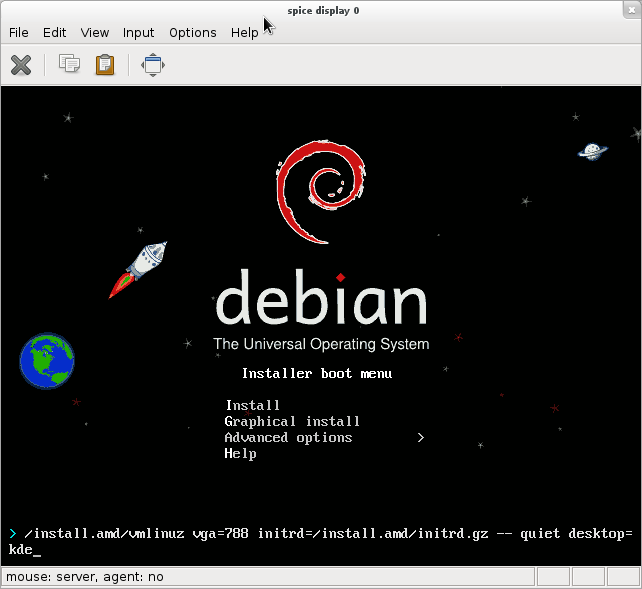
\includegraphics[width=7cm]{image201202/kdedesk/stable-inst-menu.png}
\caption{安定版インストール画面でTABキーを押したときの様子}
\end{center}
\end{figure}
\item あとは通常どおりインストールを行います。インストールを進めていくと「インストールするソフトウェアの選択:」のメニューが現れますので、''Debian desktop environment''を選択しておいてください。
\item インストールが完了しましたら、リブートを行います。
\item KDE環境が起動します。
\end{enumerate}

以上となります。簡単ですね。

\subsection{\label{sec:exp-kde}開発者としてのexperimental版KDE導入方法(KVM+spice)}

 東京エリアDebian勉強会にいらっしゃるような方々には、前述のインストールと環境では
きっと「ぬるゲー(笑)」な感じのはずです。その場合、是非とも
experimental版のKDE環境を利用いただき、BTS書き/パッチ開発/翻訳/デバッグなどの
開発活動に勤しんでみましょう。ここでは、開発者向けKDE環境導入について簡単に述べます。

\begin{itemize}
\item 開発者向けにexperimental版導入を前提にします。
\item 仮想環境であるKVMを利用して仮想環境上に導入します。これなら、ディスクイメージファイルをとっておけば、うっかりexperimental環境でaptitude full-upgradeして全く立ち上がらなくなっても(実話)あっさり復帰できます。
\item サウンドももちろん欲しいので仮想デスクトップ環境としてspiceを使います。
\item いつでもどこでも開発できるようにモバイル環境に構築します。
\end{itemize}
図\ref{fig:kde-env}のKDE開発環境の用意を想定します。

\begin{figure}[ht]
\begin{center}
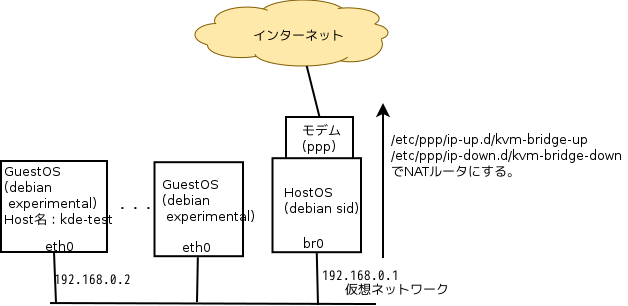
\includegraphics[width=10cm]{image201202/kdedesk/kde-dev-env.png}
\caption{\label{fig:kde-env}KDE開発環境}
\end{center}
\end{figure}

以下は導入に関しての流れです。(細かい事は割愛します。操作にあたっては適宜root権限が必要だったりします)
\begin{enumerate}
\item HostOSとなるPCのBIOSを操作して、CPUの仮想技術支援機構のスイッチをONにしてブートしておきます。
\item HostOSに\url{http://www.debian.org/CD/netinst}から名刺サイズのCDイメージを落として置きます。
\item HostOSの/etc/network/interfacesに以下の追記を行い、br0を作っておきます。
\begin{commandline}
# 追記はここから。aptitude install bridge-utilsはやっておくこと。
auto br0
iface br0 inet static
        address 192.168.0.1
        netmask 255.255.255.0
        bridge_ports none
        bridge_stp off
        bridge_fd 0
        bridge_maxwait 0
\end{commandline}
\item HostOSの/etc/sysctl.d/bridge-filter-workaround.confを作り、sysctl -p /etc/sysctl.d/bridge-filter-workaround.confを実行して、br0のフィルタを無効化しておきます。
\begin{commandline}
# /etc/sysctl.d/bridge-filter-workaround.confの中身
net.bridge.bridge-nf-call-ip6tables = 0
net.bridge.bridge-nf-call-iptables = 0
net.bridge.bridge-nf-call-arptables = 0
\end{commandline}
\item HostOSの/etc/ppp/ip-up.d/kvm-bridge-up,/etc/ppp/ip-down.d/kvm-bridge-downを作っておきます。他にフィルタとか必要であれば適当にどうぞ。
\begin{commandline}
#!/bin/sh
# /etc/ppp/ip-up.d/kvm-bridge-upの中身
PATH=/bin:/usr/bin:/sbin:/usr/sbin
CDPATH=
sysctl -w net.ipv4.ip_forward=1
iptables -t nat -A POSTROUTING -o $PPP_IFACE -j MASQUERADE
iptables -A FORWARD -i br0 -o $PPP_IFACE -j ACCEPT
\end{commandline}
\begin{commandline}
#!/bin/sh
# /etc/ppp/ip-down.d/kvm-bridge-downの中身
#!/bin/sh
PATH=/bin:/usr/bin:/sbin:/usr/sbin
CDPATH=
sysctl -w net.ipv4.ip_forward=0
iptables -t nat -D POSTROUTING -o $PPP_IFACE -j MASQUERADE
iptables -D FORWARD -i br0 -o $PPP_IFACE -j ACCEPT
\end{commandline}
\item HostOSにkvm/libvirt/spice-client-gtkパッケージを導入しておきます。
\item HostOSにてGuestOS用のkde-test.xmlを以下の雛形で作成してvirsh define kde-test.xmlしておきます。\footnote{virt-installは何故か自分のexperimentalな環境ではSegmentation Faultで落ちてしまうのでここでは使いません。BTSしときます。}
\begin{commandline}
<domain type='kvm'>
  <name>kde-test</name>
  <memory>1048576</memory>
  <vcpu>1</vcpu>
  <os>
    <type arch='x86_64' machine='pc-1.0'>hvm</type>
    <boot dev='hd'/>
    <boot dev='cdrom'/>
    <bootmenu enable='yes'/>
  </os>
  <features>
    <acpi/>
    <apic/>
    <pae/>
  </features>
  <clock offset='utc'/>
  <on_poweroff>destroy</on_poweroff>
  <on_reboot>restart</on_reboot>
  <on_crash>restart</on_crash>
  <devices>
    <emulator>/usr/bin/kvm</emulator>
    <disk type='file' device='disk'>
      <driver name='qemu' type='raw' cache='writeback'/>
      <source file='/var/lib/libvirt/images/kde-test.img'/>
      <target dev='vda' bus='virtio'/>
    </disk>
    <disk type='file' device='cdrom'>
      <driver name='qemu' type='raw'/>
<!-- directory of cdimageは適当に変更ください -->
      <source file='/directory of cdimage/debian-6.0.4-amd64-businesscard.iso'/>
      <target dev='hdc' bus='ide'/>
      <readonly/>
    </disk>
    <controller type='ide' index='0'/>
    <interface type='bridge'>
<!-- macアドレスは適当に変更ください -->
      <mac address='52:54:00:31:cd:5a'/>
      <source bridge='br0'/>
      <model type='virtio'/>
    </interface>
    <serial type='pty'>
      <target port='0'/>
    </serial>
    <console type='pty'>
      <target type='serial' port='0'/>
    </console>
    <input type='mouse' bus='ps2'/>
    <graphics type='spice' port='5900' autoport='no'>
      <clipboard copypaste='yes'/>
    </graphics>
    <sound model='ac97'\>
    <video>
      <model type='qxl' vram='9216' heads='1'/>
    </video>
    <memballoon model='virtio'>
    </memballoon>
  </devices>
</domain>
\end{commandline}
\item HostOSで仮想環境用のディスクを10GBぐらいで作っておきます。
\begin{commandline}
qemu-img create -f raw /var/lib/libvirt/images/kde-test.img 10G
\end{commandline}
\item HostOSでKVMを起動して、spiceクライアントを接続します。
\begin{commandline}
virsh start kde-test; spicy -h 127.0.0.1 -p 5900 &
\end{commandline}
\item GuestOSのDebianインストーラが起動したら、TABキーを押し、画面下に現れた編集可能な行に、''priority=medium''を以下のように入力してインストールを開始します。
\begin{commandline}
 /install.amd/vmlinuz vga=788 initrd=/install.amd/initrd.gz --- quiet priority=medium
\end{commandline}
インストール途中「Debian アーカイブのミラーを選択」のメニューにて''sid''を選択し、「インストールするコンポーネント」として「sshサーバー」のみ(他は選択しない)とします。
\item インストールが完了すると、テキストコンソールからDebian sidなGuestOSへログインできるようになります。
\item GuestOSにログインして以下の行を/etc/apt/source.listへ付け加えます
\begin{commandline}
#追加内容
deb http://ftp.jp.debian.org/debian/ experimental main
deb-src http://ftp.jp.debian.org/debian/ experimental main
\end{commandline}
\item GuestOSの/etc/apt/preference.dにDebian KDEチーム製のexperimentalパッケージ用preferenceファイルをインストールします。
\begin{commandline}
cd /etc/apt/preference.d && wget http://pkg-kde.alioth.debian.org/files/kde-experimental
\end{commandline}
\item GuestOSで以下を実行し、experimentalなKDE環境を一気に入れてしまいます。
\begin{commandline}
aptitude update;aptitude aptitude install task-kde-desktop task-japanese-kde-desktop;aptitude clean
\end{commandline}
\item インストールが終わったら、GuestOSをリブートします。GuestOSでKDEのexperimental版が起動し、グラフィカルなログイン画面が現れます。
\end{enumerate}

\subsection{DebianとKDE環境のバージョン}

DebianのバージョンとKDEのバージョンの対応を表\ref{tab:kde-ver}に載せます。

\begin{table}[ht]
\begin{center}
\begin{tabular}{|l|l|l|l|l||l|}
\hline 
Debian&stable&testing&unstable&experimental&upstream\\
\hline \hline
KDE &4.4&4.6&4.6&4.7.4&4.8.0\\
\hline
\end{tabular}
\caption{\label{tab:kde-ver}DebianのバージョンとKDEのバージョン}
\end{center}
\end{table}

KDEのupstreamは2012年1月25日に4.8.0をリリースしたばかりなので、まだ
experimentalも追いついていない状態です。

\subsection{KDE環境の開発の特徴}

KDE環境の開発は以下のような特徴があります。

\begin{enumerate}
\item Qt(キュート)ライブラリを使う。
\item C++のコードが基本
\item autotoolsの代わりにcmakeが使われる
\end{enumerate}

このため、Debianではパッケージ開発の為にpkg-kde-toolsパッケージが用意されています。

\subsection{DebianでのKDE環境のパッケージ開発}

 DebianではKDE環境のパッケージ開発用にpkg-kde-toolsというパッケージを別に用意しています。こちらを導入するとKDE環境のパッケージ構築の際に便利な機能が使えるようになります。

\begin{table}[ht]
\begin{center}
\begin{tabular}{|l|l|l|l|}
\hline 
項番&拡張されるもの&拡張&備考\\
\hline
1&dh& --with kde & debhelperにkde用の拡張を指定\\
\hline
2&dh\_auto\_*& --buildsystem=kde & dh\_auto\_*がcmakeを使うようになる、KDE環境用の設定を行う等\\
\hline
3&CDBS&kde.mk& CDBSでKDE用の拡張が利用できるようになる\\
\hline
4&その他&variables.mkなど& debian/rulesの中で\$(DEB\_CMAKE\_KDE4\_FLAGS)などが使える等\\
\hline
\end{tabular}
\caption{\label{tab:pkg-kde-tools-inst}pkg-kde-toolsをインストールした時の拡張}
\end{center}
\end{table}

\subsection{超簡易的にKDE用プログラムのDebianパッケージを作ってみる}

ここでは超簡易的にKDE用プログラムのDebianパッケージを作ってみます。

まず、事前準備として、

\begin{itemize}
\item 環境は\ref{sec:exp-kde}章のexperimental環境を用意ください。
\item  必要なパッケージ(cmakeパッケージ等)
\footnote{KDE環境向けの開発が全く初めての人は、細かい事が判ってくるまで、aptitude build-dep kdeutilsしておいてKDEパッケージ開発に必要なパッケージをあらかじめまとめて導入しておくという手もあります}
\end{itemize}

次にkhello-1.0.0/なるディレクトリに\url{http://techbase.kde.org/Development/Tutorials/First_program}にある、main.cppとCMakeLists.txtを配置します。

\begin{commandline}
$ cd khello-1.0.0
$ ls 
CMakeLists.txt main.cpp
$
\end{commandline}
% $ 

次に、オリジナルのtar.gzアーカイブを作成しておきます。

\begin{commandline}
$ cd ..
$ tar czf khello_1.0.0.orig.tar.gz khello-1.0.0
$ ls -F 
khello-1.0.0/  khello_1.0.0.orig.tar.gz
$
\end{commandline}

dh\_make を使ってdebian/ディレクトリを仕込みます。あとはrulesファイル以外
いつも通り、パッケージを作成するようにファイルを作成しておきます。

\begin{commandline}
$ cd khello-1.0.0/debian
$ ls -F
README.Debian  changelog  control    docs   source/
README.source  compat     copyright  rules
$ 
\end{commandline}
% $

pkg-kde-toolsパッケージを利用するrulesファイルを記載します。

\begin{commandline}
# pkg-kde-toolsを使ったKDE開発用debian/rulesファイルの中身。

%:
       dh $@ --with kde
\end{commandline}
%$

あとは、dpkg-buildpackage -uc -us -rfakerootを実行してビルドします。

\begin{commandline}
$ dpkg-buildpackage -us -uc -rfakeroot
dpkg-buildpackage: source package khello
...中略...
dpkg-source: info: building khello in khello_1.0.0-1.debian.tar.gz
dpkg-source: info: building khello in khello_1.0.0-1.dsc
 debian/rules build
dh build  --with kde
   dh_testdir
   dh_auto_configure --buildsystem=kde
-- The C compiler identification is GNU
-- The CXX compiler identification is GNU
...中略...
\end{commandline}
%$

 無事、--buildsystem=kdeが利用され、cmakeが実行されています。

 しばらく待つと無事にkhello\_1.0.0-1\_amd64.debなどが出来上がります。

 ほら、pkg-kde-toolsのおかげでパッケージ開発も簡単でしょ?でしょ?

\subsection{おわりに}

 今回は、Debian開発者の為のKDE環境の構築と、簡単なパッケージ作成について、
一通り記載してみました。これを機に、KDE環境に関する開発をされる方が増えると
うれしいと思っています。

\subsection{参考文献}

\begin{itemize}
\item \url{http://pkg-kde.alioth.debian.org/} Debian KDE Teamのホームページ。
\item \url{http://techbase.kde.org} KDE Techbase
\item \url{http://kde.org/} KDE本家
\item \url{http://www.spice-space.org/} SPICE仮想デスクトップデバイス本家
\end{itemize}

%-------------------------------------------------------------------------------
\dancersection{月刊Debhelper}{山本 浩之}
%-------------------------------------------------------------------------------

\index{debhelper makeまえにふかいりしてみる@debhelper make前に深入りしてみる}

\subsection{パッケージのmakeの前に…}

先月までに学んできたように、Debhelperは、基本的にビルドに必要な一連のdh\_ほげほげコマンドを自動実行します。

例えばDebhelperは、dh\_auto\_configureというコマンドを提供しており、これはご想像の通り、
\begin{commandline}
./configure --build='dpkg_architecture_value("DEB_BUILD_GNU_TYPE")' --prefix=/usr --includedir=/usr/include \
--mandir=/usr/share/man --infodir=/usr/share/info --sysconfdir=/etc --localstatedir=/var \
--libdir=/usr/lib/\$multiarch --libexecdir=/usr/lib/\$multiarch --disable-maintainer-mode \
--disable-dependency-tracking --host='dpkg_architecture_value("DEB_HOST_GNU_TYPE")
\end{commandline}
をしているだけです。

しかし、メンテナによってautotoolsを利用し、confugureスクリプトをビルドの度に毎回configure.acから生成したい人もいるでしょうし、もしかするとMakefileの元となるMakefile.inだって、毎回Makefile.amから生成したい人もいるでしょう。
また、Debianパッケージオリジナルのパッチをあててパッケージを作るのは、ごく当たり前のように行なわれています。

そこで今月は、一連のdh\_ほげほげコマンドへの追加の仕組みと、その例として、dpatchパッケージで提供されるdh\_dpatch\_patchコマンドと、autotools-devパッケージで提供されるdh\_autotools-dev\_updateconfigコマンドの追加について解説しましょう。

\subsection{一連のdh\_ほげほげコマンドへの追加の仕組み}

基本となる一連のdh\_ほげほげコマンドは、大元のコマンドであるdhスクリプトに記述してあり、すべてについては先月や先々月に話されているので、割愛します。

特にmake直前に実行されるものは、
\begin{commandline}
dh_testdir  #カレントディレクトリの確認
dh_auto_configure  #./configureの実行
\end{commandline}
だけです。

勿論、これだけではパッチもあてられないですし、configureスクリプトの再生成もできません。

そこでdhスクリプトは、一連のdh\_ほげほげコマンドを列挙する配列にし、これを\$sequences{\$sequence}のスカラ変数として保持しています。(この辺はperlにあまり詳しくないので、ちょっと間違っているかも…)

また、この\$sequencesからdh\_ほげほげコマンドを除いたり(remove\_command)、あるdh\_ほげほげコマンドの前に追加する(insert\_before)サブルーチンも用意されています。

dhスクリプトは、/usr/share/perl5/Debian/Debhelper/Sequence/ディレクトリのなかにあるファイルを参照しており、ここに
\begin{commandline}
insert_before("dh_auto_configure", "dh_追加ほげほげ")
\end{commandline}
という記述のあるファイル(アドオン)が追加されると、dh\_auto\_configureの前にdh\_追加ほげほげコマンドが実行されるようになります。

ただし、rulesの
\begin{commandline}
dh $@ --with 〜 
\end{commandline}
でアドオンが指定されない限り評価はされないので、ビルドに不必要なdh\_ほげほげコマンドを入れていても大丈夫なはずです。

\subsection{dh\_dpatch\_patchコマンド}

dpatchパッケージをインストールすると、/usr/share/perl5/Debian/Debhelper/Sequence/ディレクトリにdpatch.pmファイルが入り、これには、
\begin{commandline}
insert_before("dh_auto_configure", "dh_dpatch_patch")
insert_before("dh_clean", "dh_dpatch_unpatch")
\end{commandline}
という記述があります。これは見て想像できるとおり、makeの直前に実行される./configureのさらに直前に、dh\_dpatch\_patchを加えています。
また、下の記述は、以前にビルドしたことがある場合に、パッチする前の状態にするdh\_dpatch\_unpatchコマンドも追加されています。

このdh\_dpatch\_patchは、パッケージソースのdebian/patches/00listに記述されたファイル名のパッチを先頭からパッチするコマンド、dpatchスクリプトを実行します。

すなわち、もしconfigureスクリプトにdpatchでなんらかのパッチをあてて実行したければ、dpatchパッケージをBuild-depし、debian/patches/ディレクトリにパッチファイルとそれに合わせた00listファイルを用意し、
\begin{commandline}
dh $@ --with dpatch
\end{commandline}
とrulesファイルに記述しておけば良いはずです。

makeだけしたいならば、ターミナルで、
\begin{commandline}
$ dh_dpatch_patch
$ ./configure 〜
$ make
\end{commandline}
でも大丈夫です。

\subsection{autotoolsだって使いたい}

ビルドするマシンの環境に合わせて、configureスクリプトなどを調整してくれるツールとして、GNU autotoolsというものがあります。次にこのGNU autotoolsをDebhelperで利用する方法について述べましょう。

\index{dh-autoreconf}
dh-autoreconfパッケージをインストールすると、依存関係でautomake、autoconfと、automakeに依存してautotools-devがインストールされます。
autotools-devパッケージは/usr/share/perl5/Debian/Debhelper/Sequence/ディレクトリにautotools-dev.pmファイルが入ります。
これには、
\begin{commandline}
insert_before("dh_auto_configure", "dh_autotool-dev_updateconfig")
insert_before("dh_clean", "dh_autotool-dev_restoreconfig")
\end{commandline}
と記述されています。

dh\_autotool-dev\_updateconfigコマンドは、カレントディレクトリ以下で実行しているシステムタイプの標準名を推測するためのconfig.guessとconfig.subファイルを探し、config.guess.dh-origとconfig.sub.dh-origファイルに名前を換え、それぞれ/usr/share/misc/ディレクトリにある最新autotool-devのconfig.guessとconfig.subをコピーしてきます。

dh-autoreconfパッケージは/usr/share/perl5/Debian/Debhelper/Sequence/ディレクトリにautoreconf.pmファイルが入ります。
これには、
\begin{commandline}
insert_before("dh_auto_configure", "dh_autoreconf")
insert_before("dh_clean", "dh_autoreconf_clean")
\end{commandline}
と記述されています。

dh\_autoreconfコマンドは、簡単に言うと、automake、autoconfをしてくれるautoreconfスクリプトを呼び出し、configureやMakefile.inを再生成します。

dh\_autoreconfを使いたいときは、このパッケージにBuild-depし、
\begin{commandline}
dh $@ --with autoreconf
\end{commandline}
とrulesファイルに記述しておけば良いはずです。
debian/autoreconfファイルにディレクトリのリストがあれば、そこだけconfigureやMakefile.inを更新してくれます。

autoreconf.pmファイルでは「dh\_auto\_configureより前だよ」という指定しかありませんから、dh\_autoreconfが実行されてパッチがあてられるのか、パッチがあてられてからdh\_autoreconfが実行されるのかまでは記述されていません。
dhスクリプトを見た限りでは「--with」オプションの順でリストされているようです。つまり、dh-autoreconfパッケージを利用するソースパッケージのMakefileに対してBTSでパッチを書く場合は、「--with」オプションの順を確認する必要がありそうです。

\subsection{おわりに}

今回はmakeを実行する前に使用されるconfigureスクリプトなどの、Debhelperを使ったカスタマイズ法について、駆け足で説明してみました。

%-------------------------------------------------------------------------------
\dancersection{cmake使ってみる}{野島 貴英}
%-------------------------------------------------------------------------------

\index{cmake}

\subsection{cmakeとは}

KDE環境の開発に使われているツールにcmakeがあります。これは従来のautotools
のようなものです。が、autotoolsに比べて次に述べる代表的な特徴があります。

\begin{itemize}
\item バイナリのプログラムである\\
autotoolsは、ご存知の通り、中はshスクリプトとなっています。これは
/bin/shを基本コマンドとして持つ従来のUNIX系のOSで使うなら非常に都合がよ
いのですが、そもそも/bin/shを持たないシステムの元で利用しようとすると
動作できません。これでは、例えば、標準的なCプログラムをコンパイル出来る環境
なのに、/bin/shが無いという本質ではない理由の為に移植性を損なうのはちょっと
残念です。

 cmakeはバイナリのプログラムなので、コマンド単体で動作することができ、
/bin/shなどUNIXのコマンドが無い場所でも問題なく動作できます。

\item 様々なプラットフォーム用の構築システムに対応できる\\
 autotoolsはmakeに特化したツールとなります。ここで、そもそもMakefileが
一般的ではない開発環境(例:Microsoft Visual Studio等の様々なIDE)の場合、
MakefileよりもIDEのプロジェクトファイルを生成できた方がより都合がよかったりします。
  cmakeは一本のCMakeLists.txtを用意するだけで、Makefileや、IDE環境用
のプロジェクトファイルを生成できたりする能力があります。この為、autotoolsを
利用したソースパッケージのように、Makefile.amと、例えば.vcprojファイルを別々に
修正してUNIX/Windows間の移植性を保つというような作業から開発者が開放
される可能性を意味します。

\item その他\\
 詳しいサマリは、DDJジャーナルの\url{http://drdobbs.com/cpp/184405251}に
サマリされているような機能がある模様です(まだ自分は未評価です。)

この記事からいくつか抜粋すると、

\begin{itemize}
\item QTライブラリのmocコマンド/ITKのCABLE/VTKのラッパー生成コマンドに対応したステートメント
\item 静的ライブラリ、動的ライブラリの生成を容易に切り替えれるようにする機能
\item ファイルの依存関係の自動生成、並列ビルドのサポート
\end{itemize}

がある模様です。
\end{itemize}

\subsection{使ってみる}

百聞は一見にしかずなので、ちょっと使ってみます。

cmakeパッケージをシステムに導入します。

\begin{commandline}
aptitude install cmake
\end{commandline}

次に以下のソース(hello.c,config.h.in)を用意します。

\begin{commandline}
/*hello.c*/
#include <stdio.h>
#include "config.h"
int main(int argc,char **argv)
{
	printf("hello world\n");
#if defined(HAVE_EXIT)
	printf("yes, this system has exit()\n");
#endif
	return(0);
}
\end{commandline}
\begin{commandline}
/*config.h.in*/
#cmakedefine HAVE_EXIT
\end{commandline}

次に、CMakeLists.txtを用意します。
\begin{commandline}
# cmakeのバージョンは2.8以上
cmake_minimum_required(VERSION 2.8)
# projectの名前を宣言
project(hello)

# cmake提供のマクロをロードする。ここでは関数がシステムにあるかを確かめるマクロ
# を使ってみる。
include (${CMAKE_ROOT}/Modules/CheckFunctionExists.cmake)

# exit()関数をチェックしてみる。あればHAVE_EXITを定義せよという意味。
check_function_exists(exit HAVE_EXIT)

configure_file (
  "${PROJECT_SOURCE_DIR}/config.h.in"
  "${PROJECT_BINARY_DIR}/config.h"
)
# cc -Iに何指定するか
include_directories ("${PROJECT_BINARY_DIR}")

# helloはhello.cから出来るという事を指定
add_executable(hello hello.c)
\end{commandline}

これら3つのファイルをhello-src/以下に配置します。
\begin{commandline}
$ ls -lR
.:
合計 4
drwxr-xr-x 2 nojima nojima 4096  2月 17 03:15 hello-src

./hello-src:
合計 8
-rw-r--r-- 1 nojima nojima 46  2月 17 03:15 CMakeLists.txt
-rw-r--r-- 1 nojima nojima  34  2月 17 04:21 config.h.in
-rw-r--r-- 1 nojima nojima 91  2月 17 03:10 hello.c
$
\end{commandline}

今回はビルド用ディレクトリ(hello-build)を作り、移動します。

\begin{commandline}
$ ls 
hello-src
$ mkdir hello-build
$ cd hello-build
\end{commandline}
% $

cmakeを実行します。

\begin{commandline}
$ cmake ../hello-src
-- The C compiler identification is GNU
-- The CXX compiler identification is GNU
-- Check for working C compiler: /usr/bin/gcc
-- Check for working C compiler: /usr/bin/gcc -- works
...中略...
-- Looking for exit
-- Looking for exit - found
-- Configuring done
-- Generating done
-- Build files have been written to: /.../cmake-test/hello-build
$ ls
CMakeCache.txt  CMakeFiles  Makefile  cmake_install.cmake  config.h
\end{commandline}

自動的に環境チェックが行われMakefile/config.hが出来上がります。
exit関数も見つかったとの表示が行われました。ここでmakeしてみます。

\begin{commandline}
$ make
Scanning dependencies of target hello
[100%] Building C object CMakeFiles/hello.dir/hello.c.o
Linking C executable hello
[100%] Built target hello
$ ls -F
CMakeCache.txt  CMakeFiles/  Makefile  cmake_install.cmake  config.h  hello*
$ ./hello
hello world
yes, this system has exit()
$
\end{commandline}

CMakeLists.txtから無事に実行バイナリ(hello)が出来上がりました。また、defined(HAVE\_EXIT)もTrueとなり、exit()関数がある時のコードもコンパイルされています。

\subsection{IDE用のプロジェクトファイルを生成してみる}

cmakeを引数無しで実行すると、helpが出てきます。このヘルプの文章の中に、どんなIDE用のプロジェクトファイルを生成できるかについて説明があります。試しに手元のDebianマシンで実行すると、

\begin{commandline}
$ cmake
...中略..
The following generators are available on this platform:
  Unix Makefiles              = Generates standard UNIX makefiles.
  CodeBlocks - Unix Makefiles = Generates CodeBlocks project files.
  Eclipse CDT4 - Unix Makefiles
                              = Generates Eclipse CDT 4.0 project files.
  KDevelop3                   = Generates KDevelop 3 project files.
  KDevelop3 - Unix Makefiles  = Generates KDevelop 3 project files.
$
\end{commandline}

ここでは試しに先ほどのhello-buildディレクトリ以下でKDevelp3 project ファイルを生成してみます。

\begin{commandline}
$ cmake -G KDevelop3 ../hello-src
...中略...
$ ls 
MakeCache.txt  Makefile             config.h        hello.kdevelop.filelist
CMakeFiles     cmake_install.cmake  hello.kdevelop  hello.kdevses
$
\end{commandline}
%$
確かにKDevelp3用のプロジェクトファイル(hello.kdevelop等)が生成されています。

\subsection{おわりに}

cmakeはKDEの他にもmysqlでも採用されています。また、wikipedia(\url{http://ja.wikipedia.org/wiki/CMake})によれば、利用しているアプリケーションも続々増えている模様です。

使いこなせると強力なツールとなりそうな感じです。皆さんも使ってみてはいかがでしょうか?Debianならaptitudeで簡単に導入できますので、是非試してみてください。

\subsection{参考文献}

\begin{itemize}
\item \url{http://www.cmake.org/} cmake本家
\item \url{http://www.cmake.org/cmake/help/cmake_tutorial.html} cmakeチュートリアル
\item \url{http://drdobbs.com/cpp/184405251?pgno=1} DDJジャーナルの記事
\end{itemize}

\printindex

\cleartooddpage

\vspace*{15cm}
\hrule
\vspace{2mm}

\includegraphics[width=2cm]{image200502/openlogo-nd.eps}
\noindent \Large \bf Debian 勉強会資料\\
\noindent \normalfont \debmtgyear{}年\debmtgmonth{}月\debmtgdate{}日 \hspace{5mm}  初版第1刷発行\\
\noindent \normalfont 東京エリア Debian 勉強会 (編集・印刷・発行)\\
\hrule

\end{document}
